\documentclass{beamer} % Использование класса beamer для создания презентации
\usetheme{Boadilla} % Применение темы Boadilla

\usepackage[T2A]{fontenc} % Установка кодировки шрифта
\usepackage[utf8]{inputenc} % Установка кодировки исходного текста
\usepackage[english,russian]{babel} % Подключение локализации и переносов для русского и английского языков
\usepackage{amsmath,amssymb} % Подключение математических символов и формул
\usepackage{autonum} % Автоматическая нумерация формул только при наличии ссылок на них
\usepackage{wrapfig} % Подключение пакета для обтекания текстом рисунков и таблиц
\usepackage{array} % Подключение пакета для работы с таблицами
\usepackage{multirow} % объединение ячеек таблиц по вертикали


\newcommand{\PreserveBackslash}[1]{\let\temp=\\#1\let\\=\temp} % Команда для сохранения обратной косой черты в ячейках таблицы
\newcolumntype{C}[1]{>{\PreserveBackslash\centering}p{#1}} % Создание нового типа столбца с центрированным содержимым

\usepackage[labelformat=empty]{caption} % Подключение пакета для настройки подписей и удаление названия "Рисунок"
\graphicspath{{./images/}{./images/logo/}} % Указание папок, где искать изображения

\setbeamertemplate{navigation symbols}{} % Удаление навигационных символов на слайдах
\usepackage{ragged2e} % Подключение пакета для улучшенного выравнивания текста
\newcommand{\jj}{\righthyphenmin=20 \justifying} % Команда для активации выравнивания по ширине с установкой минимального количества символов в слове перед переносом


\begin{document}




\begin{frame}
  \begin{center}\tiny
    Национальный исследовательский университет ИТМО\\
    Факультет систем управления и робототехники
  \end{center}

  % \begin{center}
  %   
\includegraphics[width=0.15\linewidth]{emb}
  % \end{center}

  \begin{center}\tiny
    \textbf{ВЫПУСКНАЯ КВАЛИФИКАЦИОННАЯ РАБОТА \\ ПО ПРОГРАММЕ «РОБОТОТЕХНИКА И ИСКУССТВЕННЫЙ ИНТЕЛЛЕКТ»}\\
    \vspace{0.2cm}
    \textbf{НА ТЕМУ:}\\
    \vspace{0.1cm}
    \textbf{<<РАЗРАБОТКА МУЛЬТИМОДАЛЬНОГО МЕТОДА ОДОМЕТРИИ \\ ДЛЯ МОБИЛЬНЫХ РОБОТОВ ПО ДАННЫМ КАМЕРЫ И ЛИДАРА>>}
  \end{center}

  \vspace{0.3cm}

  \begin{columns}
    \begin{column}{0.50\textwidth}
      \begin{center}\tiny
        Выполнил: \\
        \vspace{0.1cm}
        \textbf{Дюжев Владислав Дмитриевич}\\
        студент группы R34353 \\
      \end{center}
    \end{column}

    \begin{column}{0.50\textwidth}
      \begin{center}\tiny
        Научный руководитель:\\
        \vspace{0.1cm}
        \textbf{Ведяков Алексей Алексеевич} \\
        к.т.н., доцент\\
        Университет ИТМО \\
      \end{center}
    \end{column}
  \end{columns}

  \vspace{0.5cm}
  \begin{center}\tiny
    Санкт-Петербург, $2025$
  \end{center}
\end{frame}




\begin{frame}{Актуальность}
  \footnotesize{

  \textbf{Актуальность.}  
  Надёжная одометрия — ключевой элемент навигации автономных систем  
  (беспилотные автомобили, дроны, мобильные роботы).  
  Классические визуальные или лидарные схемы по отдельности  
  позволяют получить высокое качество оценки положения, однако могут быть сильно подвержены искажающим факторам. 
  Мультимодальные и дифференцируемые методы позволяют объединить
  преимущества разных сенсоров и увеличить робастность.

  \vspace{0.8cm}

  \textbf{Практическая значимость.}
  \begin{itemize}
      \item Стабильная точность локализации в неоднородных условиях съёмки  
         благодаря взаимодополняемости
        изображений и лидара;
    \item Снижение требований к сенсору --- допустимо
          использовать более доступные камеры и лидары средней ценовой категории;
    \item Универсальность решения: одна и та же мультимодальная
          архитектура масштабируется под различные мобильные платформы  
          (роботы, БПЛА, беспилотные автомобили) без кардинального пересмотра
          алгоритма.
  \end{itemize}
  }
\end{frame}




\begin{frame}{Цель и задачи работы}
  \footnotesize{

  \textbf{Цель работы} -- Разработать и исследовать мультимодальный алгоритм одометрии с использованием
  данных стерео-камеры и лидара.

  \vspace{0.6cm}

  \textbf{Задачи работы:}
  \begin{itemize}
      \item Проведение аналитического обзора в области методов одометрии на основе данных
      камеры и лидара, включая способы их комбинирования.
      \item Выбор подходящего метода интеграции визуальных и лидарных данных.
      \item Реализация прототипа мультимодального алгоритма одометрии, обеспечивающего
      оценку движения мобильного робота.
      \item Проведение серии экспериментов на открытых датасетах, сравнительного анализа
      полученных результатов с раздельными схемами, а также
      другими представителями мультимодальных методов.
      \item Формирование методических рекомендаций по использованию и настройке полученного
      решения, включая потенциальные сценарии и ограничения.
  \end{itemize}
  }
\end{frame}



\begin{frame}{Обзор существующих методов одометрии}
  \footnotesize{

  \textbf{Рассмотренные в литературе подходы}

  \begin{itemize}
      \item \textbf{Визуальные (VO)}  
            \begin{itemize}
                \item ORB-SLAM, SOFT2 --- ключевые точки + групповая корректировка;  
                \item DSO --- прямая фотометрическая оптимизация;  
                \item DF-VO --- CNN-регрессия позы.
            \end{itemize}

      \item \textbf{Лидарные (LO)}  
            \begin{itemize}
                \item LOAM / KISS-ICP --- ICP + граф поз;  
                \item EfficientLO --- проекция лидара + CNN;  
                \item \item DeepLO --- лидаpная CNN одометрия.
            \end{itemize}

      \item \textbf{Мультимодальные}  
            \begin{itemize}
                \item V-LOAM --- визуальный трекинг + лидар-карта;  
                \item H-VLO--- CNN-объединение LiDAR + RGB;
                \item \textbf{DVLO} --- контекст-кластеризация LiDAR + RGB.
            \end{itemize}
  \end{itemize}
  }
\end{frame}


\begin{frame}{Выбор базового метода}
  \footnotesize{

  \textbf{Критерии отбора}
  \begin{itemize}
      \item \textbf{Открытый код} и доступность воспроизводимости;
      \item полноценная \textbf{мультимодальное объединение} LiDAR + камера;
      \item \textbf{дифференцируемость} ― возможность дальнейшего дообучения и модификации;
      \item конкурентная точность на датасете KITTI Odometry;
      \item разумные вычислительные требования (GPU  RTX 3080).
  \end{itemize}

  \vspace{0.6cm}

  \textbf{Выбранный базовый алгоритм — DVLO}  
  \begin{itemize}
      \item использование инновационного метода объединения данных;
      \item одна камера + лидар естественно расширяется до стерео;
      \item исходный код в открытом доступе.
  \end{itemize}

  \vspace{0.3cm}
  Выбор DVLO удовлетворяет всем перечисленным критериям  
  и обеспечивает надёжную отправную точку для предложенной последующей модификации.
  }
\end{frame}

\begin{frame}{Набор данных: KITTI Odometry}
  \footnotesize{

  \textbf{Общие сведения}
  \begin{itemize}
      \item 22 последовательности городской/пригородной среды (\;43км);
      \item ground-truth траектории GPS/INS доступны для Послед.\;00–10.
  \end{itemize}

  \vspace{0.4cm}

  \textbf{Используемые сенсоры}
  \begin{itemize}
      \item \textbf{LiDAR} Velodyne HDL-64E  
            \begin{itemize}\item 64 луча, 10 Гц, $360^{\circ}$ обзор\end{itemize}
      \item \textbf{Стерео-камеры} PointGrey Flea
            \begin{itemize}\item $1241\times376$ px, 10 Гц\end{itemize}
  \end{itemize}

  \vspace{0.4cm}

  \textbf{Разбиение для экспериментов}
  \begin{itemize}
      \item \textbf{Обучение}: 00–06 
      \item \textbf{Тестирование}: 07–10
  \end{itemize}

  \vspace{0.4cm}

  \textbf{Оцениваемые метрики}
  \begin{itemize}
      \item средняя относительная ошибка расстояния
            $t_{\mathrm{rel}}$ (\%);
      \item средняя относительная ошибка ориентации
            $r_{\mathrm{rel}}$ (\,$^{\circ}$/100 м).
  \end{itemize}
  }
\end{frame}

\begin{frame}{Разработанный метод: \textit{Stereo-DVLO}}
  \footnotesize{

  \textbf{Основные изменения относительно DVLO}
  \begin{itemize}
      \item \textbf{Входные данные:} лидаp + синхронизированная стереопара RGB.
      \item Лидарные точки проецируются на изображения обеих камер,
            формируя два набора 2-D признаков.
      \item \textbf{Локальное объединение}: конкатенация признаков
            перед кластерной агрегацией приводит к
           более полному описанию локального контекста.
      \item \textbf{Глобальный модуль} и итеративный блок оценки позы
            интегрированы в новую структуру модели.
  \end{itemize}

  \vspace{0.45cm}

  \textbf{Практические свойства}
  \begin{itemize}
      \item Частота работы составляет порядка 10 Гц.
      \item Схема позволяет гибко расширять архитектуру
            другими модальностями (IMU, radar, stereo-depth).
  \end{itemize}
  }
\end{frame}


\begin{frame}{Параметры обучения и динамика сходимости}
  \footnotesize
  \begin{columns}[T]
    %---------------------------------------- ЛЕВАЯ КОЛОНКА
    \begin{column}{0.48\textwidth}
      \textbf{Общие настройки}
      \begin{itemize}
        \item \textbf{Оптимизатор:} Adam $(\beta_1{=}0.9,\;\beta_2{=}0.999)$
        \item \textbf{Начальный LR:} $1{\times}10^{-3}$, эксп.\ затухание
              до $1{\times}10^{-5}$ каждые $200\,000$ шагов
        \item \textbf{Batch size:} 8
        \item \textbf{Эпох:} 300
        \item \textbf{Аппаратура:} NVIDIA RTX 3090,
      \end{itemize}
    \end{column}

    %---------------------------------------- ПРАВАЯ КОЛОНКА
    \begin{column}{0.50\textwidth}
      \centering
      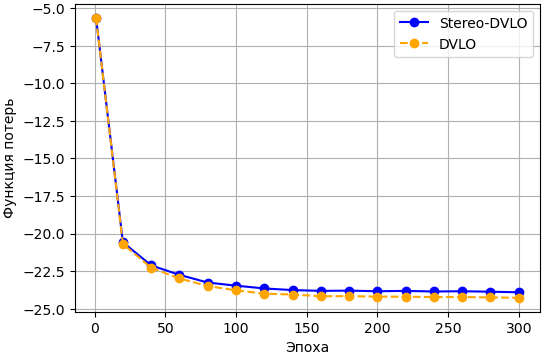
\includegraphics[width=\linewidth]{figs/loss.png}\\[4pt]
      \scriptsize
      {График функции потерь: на первых 20 эпохах
       обе модели быстро сходятся; затем плавное
       убывание c равномерным зазором между кривыми.}
    \end{column}
  \end{columns}
\end{frame}

\begin{frame}{Результаты экспериментов}
  \footnotesize

  \begin{table}
    \caption{Сравнение относительных ошибок одометрии
            на последовательностях 00–10
            (KITTI Odometry)}
      \label{tab:kitti_mono_vs_stereo}
    \begin{center}
      \begin{tabular}{|c|cc|cc|}
        \hline
        \multirow{2}{*}{Послед.} &
        \multicolumn{2}{c|}{DVLO} &
        \multicolumn{2}{c|}{Stereo-DVLO} \\
        \cline{2-5}
        & $t_{\mathrm{rel}},\;\%$ & $r_{\mathrm{rel}},\;^{\circ}/100\text{ м}$ &
          $t_{\mathrm{rel}},\;\%$ & $r_{\mathrm{rel}},\;^{\circ}/100\text{ м}$ \\ \hline
        00 & 1.08 & 0.50 & 0.99 & 0.47 \\
        01 & 1.25 & 0.47 & 1.10 & 0.36 \\
        02 & 1.55 & 0.54 & 1.01 & 0.35 \\
        03 & 0.96 & 0.46 & 1.01 & 0.81 \\
        04 & 0.67 & 0.63 & 0.61 & 0.36 \\
        05 & 1.34 & 0.62 & 0.68 & 0.34 \\
        06 & 1.00 & 0.49 & 0.37 & 0.19 \\
        07 & 1.10 & 0.69 & 0.81 & 0.47 \\
        08 & 1.73 & 0.67 & 1.32 & 0.63 \\
        09 & 1.35 & 0.56 & 1.06 & 0.48 \\
        10 & 2.31 & 1.24 & 1.09 & 0.57 \\ \hline
        \textbf{Среднее} & \textbf{1.31} & \textbf{0.62} &
        \textbf{0.91} & \textbf{0.46} \\ \hline
    \end{tabular}
    
    
    \end{center}
  \end{table}

  \vspace{6pt}

  \textbf{Итог:} стерео-модификация уменьшает средние ошибки
  расстояния на \textbf{30 \%} и средние ошибки ориентации на \textbf{26 \%} 
  без существенного изменения числа параметров модели.
\end{frame}

\begin{frame}{Траектории: последовательности 07 и 08}Пос
  \centering
  \begin{minipage}{0.48\textwidth}
    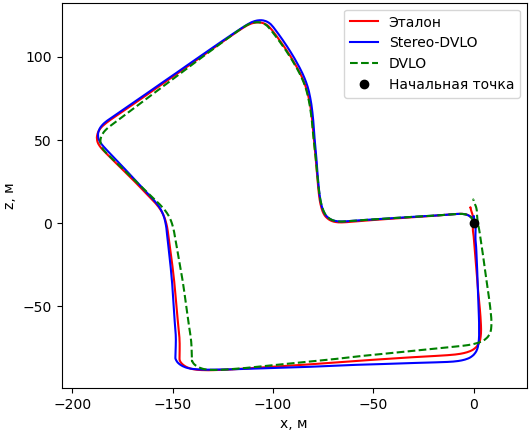
\includegraphics[width=\linewidth]{figs/07.png}\\[-2pt]
    {\scriptsize Послед.~07: сравнение работоспособности моделей DVLO и Stereo-DVLO}
  \end{minipage}\hfill
  \begin{minipage}{0.48\textwidth}
    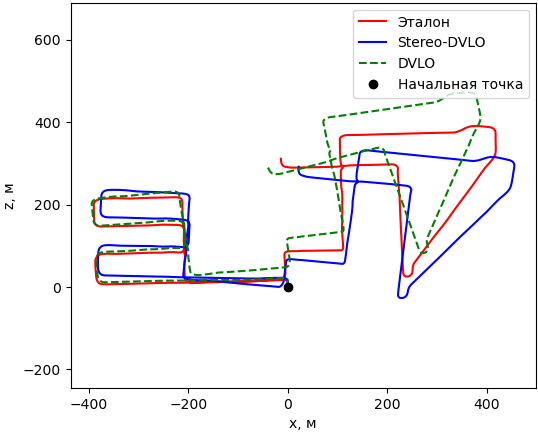
\includegraphics[width=\linewidth]{figs/08.png}\\[-2pt]
    {\scriptsize Послед.~08: сравнение работоспособности моделей DVLO и Stereo-DVLO}
  \end{minipage}
\end{frame}

\begin{frame}{Траектории: последовательности 09 и 10}
  \centering
  \begin{minipage}{0.48\textwidth}
    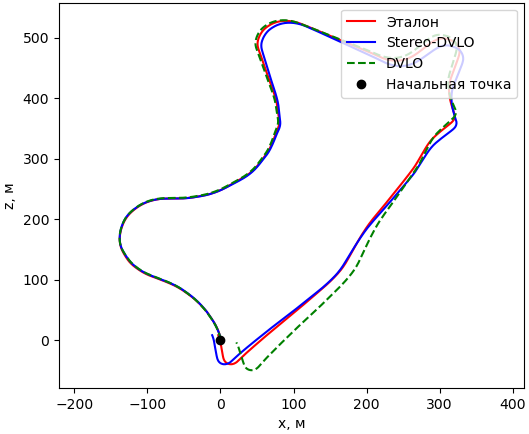
\includegraphics[width=\linewidth]{figs/09.png}\\[-2pt]
    {\scriptsize Послед.~09: сравнение работоспособности моделей DVLO и Stereo-DVLO}
  \end{minipage}\hfill
  \begin{minipage}{0.48\textwidth}
    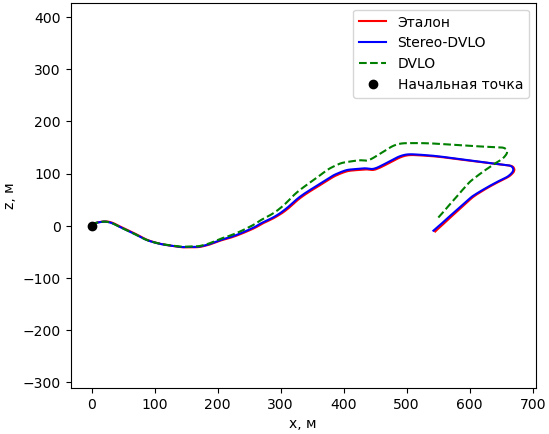
\includegraphics[width=\linewidth]{figs/10.png}\\[-2pt]
    {\scriptsize Послед.~10: сравнение работоспособности моделей DVLO и Stereo-DVLO}
  \end{minipage}
\end{frame}

\begin{frame}{Сравнение с классическими методами}
  \footnotesize
  \begin{center}
    \begin{tabular}{|l|c|c|c|c|}
      \hline
      \multirow{2}{*}{Метод} &
      \multicolumn{2}{c|}{$t_{\mathrm{rel}},\;\%$} &
      \multicolumn{2}{c|}{$r_{\mathrm{rel}},\;^{\circ}/100$\,м} \\ \cline{2-5}
      & Средн.\ & $\;\pm$\,ст.\,откл.& Средн.\ & $\;\pm$\,ст.\,откл. \\ \hline
      \textbf{Stereo-DVLO} & 0.91 & 0.23 & 0.46 & 0.13 \\
      KISS-ICP            & 0.56 & 0.19 & 0.17 & 0.02 \\
      SOFT2               & 0.62 & 0.18 & 0.19 & 0.02 \\ \hline
    \end{tabular}
  \end{center}

  \vspace{6pt}
  \textbf{Краткие выводы}
  \begin{itemize}
      \item Классические оптимизационные методы (KISS-ICP, SOFT2) достигают
            минимальных ошибок за счёт жёсткой геометрической оптимизации.
      \item Stereo-DVLO уступает по абсолютной точности, но:
            \begin{itemize}
                \item полностью дифференцируема и легко дообучается,
                      устраняя калибровочные смещения;
                \item не требует ручного подбора порогов и параметров ICP;
                \item естественно масштабируется на дополнительные сенсоры.
            \end{itemize}
  \end{itemize}
\end{frame}


\begin{frame}{Заключение}
  \footnotesize

  \begin{itemize}
      \item Выполнен анализ современных методов одометрии и выбрана
            нейросетевая база — \textbf{DVLO}.
      \item Реализована стерео-модификация, позволяющая улучшить качество оценки положения.
      \item \textbf{Результаты на KITTI Odometry}:  
            \begin{itemize}
                \item $t_{\mathrm{rel}}$: \;1.31 \%  $\rightarrow$ \textbf{0.91 \%}  
                      (требование ТЗ — не хуже 1 \%);
                \item $r_{\mathrm{rel}}$: \;0.62°/100 м $\rightarrow$ \textbf{0.46°/100 м}  
                      (требование ТЗ — не хуже 0.7°/100 м).
            \end{itemize}
      \item Сравнение с классикой (KISS-ICP, SOFT2) показало,
            что стерео-DVLO приближается к их точности,  
            оставаясь полностью дифференцируемой и менее зависимой
            от ручной калибровки.
      Таким образом, поставленные в техническом задании
            цели по снижению ошибок и демонстрации преимуществ
            нейросетевой мультимодальной одометрии \textbf{достигнуты}.
  \end{itemize}
\end{frame}


\begin{frame}
  \centering \Huge \textcolor{blue}{Ваши вопросы!}
\end{frame}


\end{document}
